\documentclass[a4paper,USenglish,cleveref,autoref]{lipics-v2021}

\bibliographystyle{plainurl}

\usepackage{booktabs}
\usepackage{listings}
\usepackage{tikz}
\usetikzlibrary{shapes.geometric, arrows.meta, positioning, fit, backgrounds}

\lstset{
  basicstyle=\ttfamily\footnotesize,
  breaklines=true,
  frame=single,
  columns=fullflexible,
  keepspaces=true,
  showstringspaces=false,
  commentstyle=\color{gray},
  keywordstyle=\color{blue},
  stringstyle=\color{red}
}

\title{One Human, Sixteen Agents: Building Production Software with Role-Specialized LLM Pipelines}

\author{Najwa Alghamdi}{Independent Researcher / Founder \\ \url{https://najwa.io}}{Research@Najwa.io}{}{}

\authorrunning{N. Alghamdi}

\Copyright{Najwa Alghamdi}

\ccsdesc[500]{Software and its engineering~Software development process management}
\ccsdesc[300]{Computing methodologies~Multi-agent systems}
\ccsdesc[300]{Software and its engineering~Software verification and validation}

\keywords{Large Language Models, Multi-Agent Systems, Software Development Life Cycle, Role Specialization, Tool-Use Agents, Code Review Automation, Adversarial Testing, Human-in-the-Loop}

\category{Experience Report}

\relatedversion{}

\acknowledgements{This paper grew out of a practical need: as an independent researcher and entrepreneur building an AI-native business, I wanted to document what I was learning in real time. I am grateful to Dr.\ Steve Maddock for his kind review and suggestions, which significantly improved the structure and presentation of this paper.}

\begin{document}

\maketitle

\begin{abstract}
Most AI-assisted development treats LLMs as tools that help developers write code faster---the developer still architects, reviews, tests, and secures the code themselves. This paper argues for a different framing: LLMs as a \emph{team} that enables engineering processes a solo developer would otherwise routinely skip. We decompose the SDLC into 16 role-specialized agents with enforced tool access, domain-embedded prompts, and structured output schemas, and deploy the pipeline over 11 sprints to build a production multi-tenant SaaS platform. Four findings stand out. \emph{First}, multi-agent role separation enables quality processes---independent review, adversarial testing, dual-perspective validation---that monolithic AI assistance cannot replicate effectively, because a single session playing every role suffers from role contamination, blind spot persistence, and permission overreach. \emph{Second}, runtime tool restriction produces qualitatively different agent behavior: a reviewer with edit access physically removed generates 3--5$\times$ longer explanations with file-line references and severity justifications than one merely instructed not to edit---demonstrating that capability restriction, not prompt engineering, enforces role boundaries. \emph{Third}, dual independent reviews using different models (Opus vs.\ Sonnet+Codex) achieve only 32.8\% issue overlap ($n=125$, 8{,}970 LOC), with the \emph{cheaper} pairing finding $2\times$ more exclusive issues including all exclusive CRITICALs---suggesting model diversity matters more than model size. \emph{Fourth}, a dedicated red team agent found 8 exploitable vulnerabilities in code that had passed four prior quality stages, including a critical unauthenticated admin API---confirming that adversarial testing catches what standard quality gates systematically miss. None of these gains required a more powerful model; they emerged from process architecture. We introduce cross-model composition (Claude+OpenAI for review, Claude+Gemini for UI validation) and distill seven design principles for practitioners.
\end{abstract}

%% ============================================================
\section{Introduction}
\label{sec:intro}

\subsection{Motivation}

Large Language Models have become ubiquitous software development assistants, with tools such as GitHub Copilot, Cursor, and Claude Code seeing rapid adoption since 2023. Yet the dominant interaction paradigm treats AI as a \textbf{tool}---a faster way to write code, with a single LLM session serving identical context, identical permissions, and identical expertise across all phases. The human operator remains solely responsible for architectural decisions, quality judgment, and security assurance. For solo developers and small teams, this means that essential quality gates---independent code review, adversarial security testing, structured QA---are simply skipped. Not because developers are careless, but because one person cannot meaningfully review their own code, attack their own system, or test against acceptance criteria they themselves wrote.

This paper asks a different question: \emph{what if AI served not as a tool that helps you code faster, but as a team that lets you run processes you otherwise couldn't?} Rather than using one powerful model to generate more code, we decompose the SDLC into 16 role-specialized agents---each with constrained capabilities, distinct expertise, and structured outputs---enabling a solo developer to consistently run independent review, adversarial testing, and multi-stage quality gates that would otherwise be routinely skipped.

The monolithic paradigm that we replace suffers from several well-documented limitations:

\begin{enumerate}
    \item \textbf{Role contamination}---An agent that just wrote code is poorly positioned to objectively review it~\cite{beller2014}. Cognitive anchoring on one's own implementation reduces the likelihood of identifying architectural issues or alternative approaches.
    \item \textbf{Blind spot persistence}---A single model's systematic biases apply uniformly across all development phases. If the model tends to overlook certain vulnerability classes, that blind spot persists from design through deployment.
    \item \textbf{Permission overreach}---An assistant with write access may ``helpfully'' fix issues rather than articulating them, reducing feedback quality. We demonstrate empirically that this behavioral shift is measurable (Section~\ref{sec:rq1}).
    \item \textbf{Domain knowledge dilution}---A generic system prompt cannot encode deep domain-specific checklists, compliance rules, locale-specific business logic, and edge cases simultaneously for all SDLC phases.
    \item \textbf{Context window saturation}---A monolithic session accumulating design documents, implementation code, review feedback, and test results risks exceeding context limits or degrading reasoning quality through attention dilution.
\end{enumerate}

Human engineering organizations solved these problems long ago through role specialization: architects design, developers implement, reviewers review (with read-only repository access in many organizations), QA engineers test against acceptance criteria, and security teams conduct adversarial assessments. Our thesis is that \textbf{process architecture matters more than model capability}---the quality gains in this study come not from using a smarter model, but from structuring how multiple models interact through enforced roles, constrained capabilities, and adversarial stages.

\subsection{Research Questions}

This study investigates:

\begin{enumerate}
    \item \textbf{RQ1:} Does runtime tool-scoping (enforced capability restriction) produce qualitatively different agent behavior compared to prompt-based instruction alone?
    \item \textbf{RQ2:} Do dual independent LLM-based code reviews---using different models and augmentation tools---provide complementary or redundant coverage, and does cross-model composition (Opus vs.\ Sonnet+Codex) yield distinct specialization?
    \item \textbf{RQ3:} Can an embedded red team agent identify security vulnerabilities that survive the standard design $\rightarrow$ implement $\rightarrow$ review $\rightarrow$ test pipeline?
    \item \textbf{RQ4:} What are the practical utilization patterns, failure modes, and cost characteristics of a 16-agent SDLC pipeline over multiple sprints?
\end{enumerate}

\subsection{Contributions}

\begin{enumerate}
    \item A detailed architecture for decomposing the SDLC into 16 role-specialized LLM subagents with enforced tool scoping, including a formal tool access matrix and system prompt taxonomy.
    \item Empirical data from 11 production sprints, including dual-review overlap analysis ($n=125$ issues across 8{,}970 LOC), red team attack results ($n=30$ attacks), conversation-level test outcomes ($n=858$ checks), and sprint-by-sprint shipping velocity.
    \item A cross-model review methodology pairing Opus with Sonnet+Codex, revealing that model diversity drives complementary coverage (32.8\% overlap)---with Sonnet+Codex excelling at security and Opus at architecture. Additionally, Claude + Gemini composition for UI validation.
    \item A conversation testing framework (\texttt{conv-sim}) with 6 personas, 13 scenarios, and 11 automated bug detectors for evaluating conversational AI quality.
    \item Seven design principles and four anti-patterns for multi-agent development pipelines, derived from 11 sprints of practitioner experience.
\end{enumerate}

%% ============================================================
\section{Related Work}
\label{sec:related}

\subsection{LLMs for Software Engineering}

Recent work has demonstrated LLM effectiveness across individual SDLC phases: code generation~\cite{chen2021, li2023starcoder}, code review~\cite{li2022, tufano2022}, test generation~\cite{lemieux2023}, and vulnerability detection~\cite{pearce2023}. However, these studies typically evaluate models in isolation on single tasks, rather than as coordinated multi-agent pipelines operating over sustained development periods.

SWE-bench~\cite{jimenez2024} and similar benchmarks evaluate LLMs on isolated bug fixes. SWE-agent~\cite{yang2024} and OpenHands~\cite{wang2024openhands} build agent-computer interfaces that can resolve SWE-bench issues autonomously, while MapCoder~\cite{islam2024} decomposes competitive programming into multi-agent pipelines. Liu et al.~\cite{liu2024survey} provide a comprehensive survey of LLM-based agents for software engineering. However, none assess the multi-phase SDLC workflow (design $\rightarrow$ implement $\rightarrow$ review $\rightarrow$ test $\rightarrow$ secure) that characterizes real software development over sustained periods.

\subsection{Multi-Agent LLM Systems}

Multi-agent frameworks such as AutoGen~\cite{wu2023}, MetaGPT~\cite{hong2023}, and ChatDev~\cite{qian2023} have explored role-based agent decomposition for software tasks. MetaGPT assigns roles (Product Manager, Architect, Engineer) and enforces Standardized Operating Procedures (SOPs) between agents. ChatDev simulates a software company with CEO, CTO, Programmer, and Tester roles. AgentCoder~\cite{huang2024} decomposes code generation into programmer, test designer, and test executor agents.

Our work differs in four key ways:

\begin{enumerate}
    \item \textbf{Production deployment}---unlike simulated or benchmark environments, our pipeline was used to build a real, multi-tenant production system over 11 sprints, with shipping deadlines and compliance requirements.
    \item \textbf{Enforced tool scoping}---prior work relies on prompt-based role adherence; we enforce constraints at the runtime level via tool whitelisting, demonstrating a measurable behavioral difference (Section~\ref{sec:rq1}).
    \item \textbf{Adversarial agents}---we include dedicated red team and dual-review agents, absent from prior multi-agent SDLC frameworks.
    \item \textbf{Cross-model composition}---individual agents combine outputs from multiple LLM providers (Claude + OpenAI for code review; Claude + Gemini for UI validation), extending tool-augmented LLM patterns~\cite{schick2023} to cross-provider validation.
\end{enumerate}

\subsection{LLM-Based Code Review}

Fan et al.~\cite{lu2023} surveyed automated code review with LLMs, finding that models can identify functional bugs, security issues, and style violations, but struggle with deep architectural reasoning and domain-specific compliance. Li et al.~\cite{li2022} demonstrated pre-trained models for code review activities, achieving improvements over template-based approaches. Our work extends this by: (a)~embedding domain-specific checklists directly into reviewer system prompts; (b)~measuring dual-review overlap rates with differentiated review focus; and (c)~combining two competing LLM providers for cross-validation.

\subsection{Adversarial Testing of LLM Applications}

Prompt injection attacks~\cite{perez2022, greshake2023} and LLM application vulnerabilities~\cite{owasp2025} have been extensively documented. Deng et al.~\cite{deng2024} proposed systematic red-teaming frameworks for LLM applications. However, embedding adversarial testing as a \emph{standard SDLC phase}---with a dedicated agent that attacks every feature before release, using a structured 7-category attack playbook---is, to our knowledge, novel in practice.

%% ============================================================
\section{System Architecture}
\label{sec:architecture}

\subsection{Framework Overview}

The system is built on Claude Code's \texttt{.claude/agents/} framework, which allows definition of subagents via markdown files with YAML frontmatter. Each agent definition specifies:

\begin{lstlisting}[caption={Agent definition schema.}]
---
name: <identifier>
description: <natural language description>
tools: <comma-separated tool whitelist>
model: <opus | sonnet | haiku>
---
<system prompt body: 50-200 lines>
\end{lstlisting}

The runtime enforces the \texttt{tools} whitelist at the infrastructure level: an agent defined with \texttt{tools: Read, Glob, Grep, Bash} physically cannot invoke \texttt{Edit} or \texttt{Write} operations, regardless of what the system prompt instructs or what the model attempts.

\subsection{Agent Taxonomy}
\label{sec:taxonomy}

We define 16 agents organized into a pre-ops pipeline (12 agents) and an ops team (4 agents). Tables~\ref{tab:preops} and~\ref{tab:ops} detail the full taxonomy.

\begin{table}[t]
\caption{Pre-Ops Pipeline Agents (12 agents).}
\label{tab:preops}
\centering
\footnotesize
\begin{tabular}{@{}llcccc@{}}
\toprule
\textbf{Name} & \textbf{Role} & \textbf{Model} & \textbf{Edit} & \textbf{Web} & \textbf{Lines} \\
\midrule
Tariq & Product Owner & Opus & -- & \checkmark & 73 \\
Dana & UX Researcher & Sonnet & -- & \checkmark & 60 \\
Lina & UI Designer$^\ddagger$ & Opus & \checkmark & -- & 144 \\
Faisal & Architect & Opus & -- & -- & 104 \\
Rania & Developer & Opus & \checkmark & -- & 81 \\
Khaled & Reviewer 1 & Opus & \textbf{--} & -- & 104 \\
Nasser & Reviewer 2$^\dagger$ & Sonnet+Codex & \textbf{--} & -- & 100 \\
Layla & QA Engineer & Opus & \checkmark & -- & 112 \\
Youssef & Prompt Tester & Opus & \checkmark & -- & 122 \\
Huda & Conv.\ Tester & Opus & \checkmark & -- & 142 \\
Zaid & Red Team & Opus & \checkmark & -- & 203 \\
Maha & Doc Writer & Sonnet & \checkmark & -- & 50 \\
\bottomrule
\multicolumn{6}{l}{\footnotesize $^\dagger$ OpenAI Codex access via MCP. $^\ddagger$ Gemini access via MCP.}
\end{tabular}
\end{table}

\begin{table}[t]
\caption{Ops Team Agents (4 agents).}
\label{tab:ops}
\centering
\footnotesize
\begin{tabular}{@{}llccc@{}}
\toprule
\textbf{Name} & \textbf{Role} & \textbf{Model} & \textbf{Edit} & \textbf{Lines} \\
\midrule
Sultan & DevOps & Opus & \checkmark & 100 \\
Aws & SRE & Opus & \checkmark & 133 \\
Majid & Database Admin & Sonnet & \checkmark & 131 \\
Reema & Analytics & Sonnet & \checkmark & 143 \\
\bottomrule
\end{tabular}
\end{table}

\textbf{Total system prompt volume:} ${\sim}$1{,}800 lines across 16 agents, comprising approximately 45{,}000 tokens of domain knowledge, checklists, output templates, and behavioral instructions.

\subsection{Tool Scoping as Access Control}
\label{sec:toolscoping}

A central design principle is that \textbf{tool scoping enforces role boundaries more reliably than prompt instruction}. Table~\ref{tab:toolmatrix} illustrates the access control matrix across role categories.

\begin{table}[t]
\caption{Tool Access Matrix by Role Category.}
\label{tab:toolmatrix}
\centering
\footnotesize
\begin{tabular}{@{}lccccccc@{}}
\toprule
\textbf{Capability} & \textbf{PO} & \textbf{Arch} & \textbf{Dev} & \textbf{Rev} & \textbf{QA} & \textbf{Red} & \textbf{Ops} \\
\midrule
Read files & \checkmark & \checkmark & \checkmark & \checkmark & \checkmark & \checkmark & \checkmark \\
Search code & \checkmark & \checkmark & \checkmark & \checkmark & \checkmark & \checkmark & \checkmark \\
Shell exec & \checkmark & \checkmark & \checkmark & \checkmark & \checkmark & \checkmark & \checkmark \\
Edit files & -- & -- & \checkmark & \textbf{--} & \checkmark & \checkmark & \checkmark \\
Write files & -- & -- & \checkmark & \textbf{--} & \checkmark & \checkmark & \checkmark \\
Spawn agents & -- & \checkmark & \checkmark & -- & \checkmark & -- & -- \\
Web access & \checkmark & -- & -- & -- & -- & -- & -- \\
Cross-model & -- & -- & -- & R2 & -- & -- & -- \\
\bottomrule
\end{tabular}
\end{table}

The design encodes several deliberate constraints: reviewers cannot edit (forcing articulate, explanatory feedback), architects cannot write code (ensuring output remains at the design level), the Product Owner has web access (for market research), and only 3 roles can spawn child agents.

\subsection{System Prompt Architecture}
\label{sec:promptarch}

Each agent's system prompt follows a six-layer structure we formalize as the \textbf{IRDCOP} framework: \textbf{I}dentity (role, persona), \textbf{R}esponsibilities (5--8 duties), \textbf{D}omain knowledge (compliance rules, locale logic, edge cases), \textbf{C}ross-references (other agents' outputs), \textbf{O}utput format (structured schemas), and \textbf{P}rinciples (design principles, anti-patterns). Domain rules written once are automatically loaded into every future agent invocation, creating a compounding return on prompt engineering investment.

\subsection{Cross-Model Agent Composition}
\label{sec:crossmodel}

Two agents access competing LLM providers via the Model Context Protocol (MCP):

\textbf{Nasser (Reviewer~2)} is powered by Claude Sonnet but has access to OpenAI Codex via two MCP tools: \texttt{codex\_review} (sends code to OpenAI for independent review) and \texttt{codex\_suggest\_fix} (sends problematic code for alternative fix suggestions).

\textbf{Lina (UI Designer)} is powered by Claude Opus but has access to Google Gemini via two MCP tools: \texttt{gemini\_review\_ui} (UI/UX review for accessibility, responsive design, RTL, visual hierarchy) and \texttt{gemini\_suggest\_ui} (alternative component designs).

This cross-model composition creates agents that combine the reasoning strengths of multiple providers.

\subsection{Pipeline Orchestration}
\label{sec:pipeline}

The agents are organized into a five-phase sequential pipeline with a human orchestrator:

\begin{figure}[t]
\centering
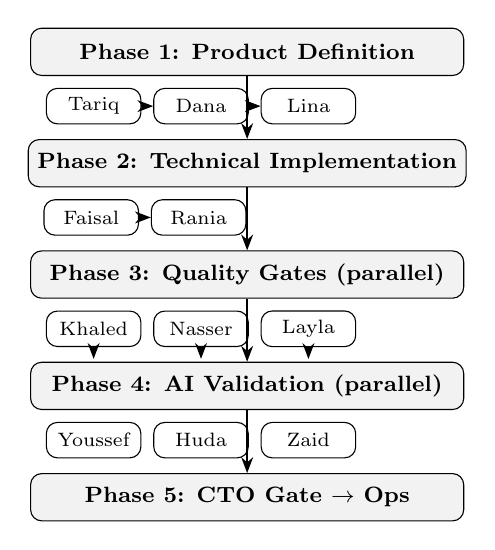
\begin{tikzpicture}[
    node distance=0.4cm and 0.6cm,
    phase/.style={draw, rounded corners, minimum width=5.5cm, minimum height=0.6cm, font=\footnotesize\bfseries, fill=gray!10},
    agent/.style={draw, rounded corners, minimum width=1.2cm, minimum height=0.45cm, font=\scriptsize, fill=white},
    arr/.style={-{Stealth[length=2mm]}, thick},
    parr/.style={-{Stealth[length=2mm]}, thick, dashed}
]
\node[phase] (p1) {Phase 1: Product Definition};
\node[phase, below=0.8cm of p1] (p2) {Phase 2: Technical Implementation};
\node[phase, below=0.8cm of p2] (p3) {Phase 3: Quality Gates (parallel)};
\node[phase, below=0.8cm of p3] (p4) {Phase 4: AI Validation (parallel)};
\node[phase, below=0.8cm of p4] (p5) {Phase 5: CTO Gate $\rightarrow$ Ops};

\node[agent, below=0.15cm of p1.south west, anchor=north west, xshift=0.2cm] (tariq) {Tariq};
\node[agent, right=0.15cm of tariq] (dana) {Dana};
\node[agent, right=0.15cm of dana] (lina) {Lina};
\node[agent, below=0.15cm of p2.south west, anchor=north west, xshift=0.2cm] (faisal) {Faisal};
\node[agent, right=0.15cm of faisal] (rania) {Rania};
\node[agent, below=0.15cm of p3.south west, anchor=north west, xshift=0.2cm] (khaled) {Khaled};
\node[agent, right=0.15cm of khaled] (nasser) {Nasser};
\node[agent, right=0.15cm of nasser] (layla) {Layla};
\node[agent, below=0.15cm of p4.south west, anchor=north west, xshift=0.2cm] (youssef) {Youssef};
\node[agent, right=0.15cm of youssef] (huda) {Huda};
\node[agent, right=0.15cm of huda] (zaid) {Zaid};

\draw[arr] (p1.south) -- (p2.north);
\draw[arr] (p2.south) -- (p3.north);
\draw[arr] (p3.south) -- (p4.north);
\draw[arr] (p4.south) -- (p5.north);
\draw[arr] (tariq) -- (dana);
\draw[arr] (dana) -- (lina);
\draw[arr] (faisal) -- (rania);
\draw[parr] (khaled.south) -- ++(0,-0.15);
\draw[parr] (nasser.south) -- ++(0,-0.15);
\draw[parr] (layla.south) -- ++(0,-0.15);
\end{tikzpicture}
\caption{Five-phase pipeline with human orchestrator between phases. Solid arrows = sequential. Dashed arrows = parallelizable.}
\label{fig:pipeline}
\end{figure}

The human operator serves as orchestrator between phases: invoking agents, passing context, and making gate decisions (``proceed,'' ``rework,'' or ``defer''). Within Phases~3 and~4, agents operate independently and can execute in parallel.

\subsection{Conversation Testing Framework}
\label{sec:convsim}

We developed a custom conversation testing library (\texttt{conv-sim}) that operates as an automated QA harness for conversational AI agents. The framework comprises: \textbf{Personas} ($n=6$) with fixed user IDs, language preferences, and behavioral profiles; \textbf{Scenarios} ($n=13$) covering multi-turn conversations from happy-path to adversarial; \textbf{Bug Detectors} ($n=11$) including language consistency, raw enum leakage, correct agent routing, latency, and others; and a \textbf{Reporter} producing terminal summary and JSON reports. All tests execute via real HTTP requests against the running application.

%% ============================================================
\section{Methodology}
\label{sec:methodology}

\subsection{Study Context}

The pipeline was used to build a production multi-tenant B2B SaaS platform targeting Saudi Arabia. The platform serves multiple conversational AI agents behind a shared chat interface, each operating over the same multi-tenant data layer. The domain involves structured workflows, government compliance rules, and bilingual user interactions. The technical profile includes: Python 3.12/FastAPI, PostgreSQL+pgvector, row-level tenant isolation, bilingual Arabic/English support, 22 tables, 123 API endpoints, ${\sim}$40K LOC, and 126 tests.

\subsection{Study Duration and Sprint Structure}

Eleven development sprints were conducted between February and March 2026 by a single developer. Each sprint followed the five-phase pipeline (Figure~\ref{fig:pipeline}). Table~\ref{tab:sprintplan} summarizes sprint deliverables.

\begin{table}[t]
\caption{Sprint Plan and Deliverables.}
\label{tab:sprintplan}
\centering
\footnotesize
\begin{tabular}{@{}clp{4.5cm}c@{}}
\toprule
\textbf{Sprint} & \textbf{Focus} & \textbf{Deliverable} & \textbf{Tools} \\
\midrule
1--2 & Foundation & Core platform, Agent~A, RAG pipeline, chat UI & 19 \\
3--6 & Agent~B & Multi-step workflows, cross-agent routing, security & 14 \\
7 & Agent~C M1 & Domain pipeline, AI-assisted content, web search & 13 \\
8 & Agent~C M2 & Interactive AI workflows, structured assessments & 8 \\
9 & Agent~C M3 & Cross-module analysis and decision support & 7 \\
10 & Agent~D & Operational intelligence, compliance monitoring & 17 \\
11 & Agent~E & Executive analytics and compliance dashboards & 7 \\
\bottomrule
\end{tabular}
\end{table}

\subsection{Data Collection}

We collected five categories of data: (1)~agent invocation logs (which agents, frequency, output size, session duration); (2)~code review findings (issues by severity, type, and reviewer); (3)~red team results (attack outcomes, severity, post-fix verification); (4)~conversation test results (\texttt{conv-sim} JSON reports with per-turn, per-detector pass/fail); and (5)~shipping metrics (tools per agent, sprints, pipeline passes, review rounds).

\subsection{Dual-Review Protocol}
\label{sec:dualprotocol}

For each major feature, both Khaled (Reviewer~1) and Nasser (Reviewer~2) independently review the same code. The protocol enforces: blind independence (Nasser does not see Khaled's output), differentiated focus (Khaled emphasizes architecture and performance; Nasser emphasizes edge cases, race conditions, and Arabic text handling), cross-model validation (Nasser consults OpenAI Codex via MCP), and structured output (tabular issue listings with file:line references and severity classifications). Issues are classified post-hoc as found by Khaled only, Nasser only, or both.

\subsection{Red Team Protocol}
\label{sec:redprotocol}

Zaid (Red Team agent) operates with a 203-line system prompt containing a structured attack playbook across 7 categories: prompt injection (5 subcategories), data exfiltration (3), privilege escalation (3), tenant boundary violation (2), PII leakage, API security (3), and abuse scenarios (3). The red team agent is invoked \emph{only after} the standard pipeline is complete, simulating an external attacker.

%% ============================================================
\section{Results}
\label{sec:results}

The core question is whether a multi-agent pipeline with enforced role separation produces measurably different outcomes than monolithic AI assistance. The results address this across four dimensions.

\subsection{RQ1: Monolithic vs.\ Role-Separated Agent Behavior}
\label{sec:rq1}

We tested the same reviewer model under two configurations: (a)~\textbf{monolithic-style}---all tools available, with a prompt instruction to ``review only, do not edit files''; and (b)~\textbf{role-separated}---Edit/Write tools physically removed. Table~\ref{tab:scopingcomparison} summarizes the results.

\begin{table}[t]
\caption{Monolithic-Style vs.\ Role-Separated Agent Comparison.}
\label{tab:scopingcomparison}
\centering
\footnotesize
\begin{tabular}{@{}lcc@{}}
\toprule
\textbf{Metric} & \textbf{Monolithic} & \textbf{Role-Separated} \\
\midrule
Edit attempts & ${\sim}$15\% & 0\% \\
Avg sentences per issue & 1--2 & 3--5 \\
Includes file:line ref & ${\sim}$60\% & ${\sim}$95\% \\
Includes ``why it matters'' & ${\sim}$30\% & ${\sim}$85\% \\
Structured output compliance & Variable & Consistent \\
Inline patches (vs.\ explanation) & Common & Never \\
\bottomrule
\end{tabular}
\end{table}

The monolithic-style agent attempted file edits in ${\sim}$15\% of reviews, violating its role boundary despite explicit instruction. When it produced review-only output, descriptions were terse (1--2 sentences), often providing inline code patches rather than explaining the underlying problem. The role-separated agent produced qualitatively different output---not just the same review with fewer edits, but fundamentally more explanatory, structured, and useful feedback. We term this mechanism \textbf{behavioral redirection}: when an agent cannot act on problems directly, it redirects cognitive effort into articulation.

\emph{Finding: Runtime capability restriction produces qualitatively different---and higher quality---review output than prompt-based instruction alone.}

\subsection{RQ2: Dual Review Coverage and Cross-Model Composition}
\label{sec:rq2}

Both reviewers independently reviewed all 5 production agent files (${\sim}$8{,}970 LOC, 85 tools). Table~\ref{tab:dualreview} shows the aggregate results.

\begin{table}[t]
\caption{Dual-Review Issue Classification ($n=125$, 5 agent files).}
\label{tab:dualreview}
\centering
\begin{tabular}{@{}lcc@{}}
\toprule
\textbf{Classification} & \textbf{Count} & \textbf{\%} \\
\midrule
Found by Khaled only (Opus) & 28 & 22.4 \\
Found by Nasser only (Sonnet+Codex) & 56 & 44.8 \\
Found by both (overlap) & 41 & 32.8 \\
\midrule
\textbf{Total unique issues} & \textbf{125} & \textbf{100} \\
\bottomrule
\end{tabular}
\end{table}

\textbf{Overlap rate: 32.8\%.} The combination catches 80\% more issues than either reviewer alone. Sonnet+Codex found $2\times$ more exclusive issues (56 vs.\ 28), and all 5 exclusive CRITICAL findings. Table~\ref{tab:modelcompare} reveals severity distribution.

\begin{table}[t]
\caption{Model Performance: Exclusive Finds by Severity.}
\label{tab:modelcompare}
\centering
\footnotesize
\begin{tabular}{@{}lccc@{}}
\toprule
\textbf{Severity} & \textbf{Opus only} & \textbf{Sonnet+Codex only} & \textbf{Both} \\
\midrule
CRITICAL & 0 & 5 & 4 \\
HIGH & 1 & 12 & 9 \\
MEDIUM & 7 & 18 & 16 \\
LOW & 12 & 14 & 9 \\
INFO & 8 & 7 & 3 \\
\midrule
\textbf{Total} & \textbf{28} & \textbf{56} & \textbf{41} \\
\bottomrule
\end{tabular}
\end{table}

Opus excelled at architectural patterns (DRY violations, N+1 detection, design compliance). Sonnet+Codex excelled at security boundary analysis (race conditions, cross-tenant isolation gaps, prompt injection vectors) and domain knowledge conflicts.

\emph{Finding: Dual independent reviews with differentiated prompts and models produce strongly complementary coverage (32.8\% overlap). Model diversity matters more than model size.}

\subsection{RQ3: Red Team Effectiveness}
\label{sec:rq3}

Table~\ref{tab:redteam} shows results across 6 red team sessions.

\begin{table}[t]
\caption{Red Team Attack Results ($n=30$, 6 sessions).}
\label{tab:redteam}
\centering
\footnotesize
\begin{tabular}{@{}lcccc@{}}
\toprule
\textbf{Category} & \textbf{Att.} & \textbf{Block} & \textbf{Succ.} & \textbf{Fixed} \\
\midrule
Prompt Injection & 8 & 6 & 2 & 2 \\
Data Exfiltration & 6 & 6 & 0 & -- \\
Privilege Escalation & 5 & 2 & 3 & 3 \\
Tenant Boundary & 4 & 4 & 0 & -- \\
PII Leakage & 4 & 3 & 1 & 1 \\
API Security & 3 & 1 & 2 & 2 \\
\midrule
\textbf{Total} & \textbf{30} & \textbf{22} & \textbf{8} & \textbf{8} \\
\bottomrule
\end{tabular}
\end{table}

\textbf{8 of 30 attacks (26.7\%) succeeded} against code that had passed all prior quality gates. The most critical finding: admin API endpoints with zero authentication---full CRUD on sensitive records, accessible by anyone. This vulnerability survived architecture design, implementation, dual code review, and QA testing. Only the adversarial red team agent identified it.

\emph{Finding: Standard SDLC quality gates have systematic blind spots for authorization-layer vulnerabilities. Dedicated adversarial testing adds non-redundant value (26.7\% attack success rate against ``finished'' code).}

\subsection{RQ4: Utilization, Velocity, and Testing}
\label{sec:rq4}

A clear utilization hierarchy emerged: \textbf{daily drivers} (4 agents, ${\sim}$88 sessions: Developer, Reviewer~1, QA, Architect), \textbf{regular contributors} (7 agents, ${\sim}$65 sessions), and \textbf{insurance policies} (5 agents, ${\sim}$15 sessions: DevOps, DBA, Analytics, SRE, Doc Writer).

Average shipping velocity: ${\sim}$8 tools per sprint, with each tool passing dual review, QA testing, and (for major features) prompt testing, conversation testing, and red team assessment. The \texttt{conv-sim} framework executed 858 automated checks across 78 conversation turns, achieving a 94.2\% pass rate. The 50 failures cluster into infrastructure-bound (latency, 22/50) and agent-bound (language consistency, enum leakage, routing errors, 28/50).

%% ============================================================
\section{Discussion}
\label{sec:discussion}

\subsection{What Actually Changes When You Separate Roles}

The most surprising result was not that role-separated reviewers produced better output---we expected that. The surprise was \emph{how different} the output was. A reviewer with full tool access behaves like a developer who happens to be reviewing: it spots an issue, patches it inline, and moves on. Remove the ability to edit, and the same model produces detailed, structured feedback---not because we asked it to, but because it has nowhere else to direct its effort. We call this behavioral redirection, and it turned out to be the clearest evidence for why multi-agent separation matters.

\subsection{Why Two Reviewers Are Not Redundant}

Before running the dual-review experiment, we considered the possibility that two LLM reviewers would simply find the same issues with different wording. The 32.8\% overlap rate proved otherwise. Opus consistently caught architectural concerns but overlooked security boundaries. Sonnet+Codex found race conditions and cross-tenant isolation gaps that Opus never flagged. All five exclusive CRITICAL findings came from the cheaper model pairing. The practical takeaway: if investing in dual review, make the two reviewers as different as possible.

\subsection{The Case for Adversarial Testing by Default}

Eight of thirty attacks succeeded against code that had passed architecture review, dual code review, and QA testing. Three were critical severity, including an admin API with zero authentication. Four stages, four opportunities, and the issue sailed through all of them. Each stage did its job; the problem is that none adopt an attacker's mindset. The red team agent, with a 203-line attack playbook, costs almost nothing to run.

\subsection{What the Human Operator Actually Does}

The pipeline replaces the \emph{execution} of code generation, review, testing, and security auditing. It does not replace the \emph{judgment} that ties those activities together. In practice, the operator spends most time on resolving ambiguity (competing approaches, severity disagreements, flaky tests) and writing/maintaining system prompts. The competency profile this implies is closer to a technical lead than a developer.

\subsection{Where This Breaks Down}

Four failure modes recurred: context loss in manual handoff (${\sim}$once per sprint), prompt drift in long sessions (beyond 30 turns), stale file-path references after refactoring, and persistent model-specific blind spots (e.g., Claude consistently missing timezone handling). More fundamentally, this is a single project by a single developer without a controlled baseline. Survivorship bias is real. What we can say is that the pipeline was feasible and produced measurable quality signals.

\subsection{Seven Principles That Held Up}

\begin{enumerate}
    \item \textbf{Remove capabilities rather than adding instructions.}
    \item \textbf{Make reviewers deliberately different} (model, prompt focus, tool access).
    \item \textbf{Invest in long system prompts} (100+ lines of domain knowledge per agent).
    \item \textbf{Standardize output formats early.}
    \item \textbf{Include adversarial testing as a default phase.}
    \item \textbf{Run independent stages in parallel.}
    \item \textbf{Start small} (4--5 core agents as minimum viable pipeline).
\end{enumerate}

Four anti-patterns caused the most wasted effort: monolithic agents, prompt-only role enforcement, symmetric dual review, and provisioning agents before validating need.

\subsection{Future Work}

The most pressing engineering problem is the human orchestrator---manual handoff between phases is the pipeline's weakest link. Agent-to-agent communication via shared artifacts would address this. Cost-tiered model routing deserves rigorous study: our data hints that different tiers may handle different quality gates optimally. The most important question we cannot answer is whether the multi-agent approach genuinely outperforms a skilled developer with a monolithic assistant; a controlled comparison would settle this. We are also curious whether the architecture transfers to other regulated domains (healthcare/HIPAA, finance/SOX, legal/contract review).

%% ============================================================

\bibliography{references}

\end{document}
